% Fig. 1 of the paper: schematic cross-section of a marine-terminated glacier.
% Build: pdflatex fig_01_schematic.tex  (needs TikZ, bm and the standalone class)
\documentclass[tikz,border=2pt]{standalone}
\usepackage{times}   % the text font of the Copernicus class
\usepackage{bm}
\usetikzlibrary{arrows.meta}
% notation macros of the paper
\newcommand{\subs}[1]{_{\mathrm{#1}}}
\newcommand{\fl}{\subs{f}}
\newcommand{\gr}{\subs{g}}
\newcommand{\gl}{\subs{gl}}
\newcommand{\cf}{\subs{cf}}
\newcommand{\wl}{\subs{wl}}
\newcommand{\basal}{\subs{b}}
\newcommand{\surf}{\subs{s}}
\newcommand{\ext}{\subs{ext}}
% colours of the paper
\definecolor{color_bed}{RGB}{184,136,119}
\definecolor{color_sea}{RGB}{168,202,221}
\definecolor{color_ice}{RGB}{236,240,241}
\definecolor{color_flat}{RGB}{108,47,138}
\definecolor{blue_custom}{RGB}{42,120,214}
\begin{document}
% Schematic cross-section of a marine-terminated glacier along the flow (Sect. 2).
% Geometry (in cm): bed, grounded ice on 0 < x < 3.5, floating ice on 3.5 < x < 5.75, ocean beyond.
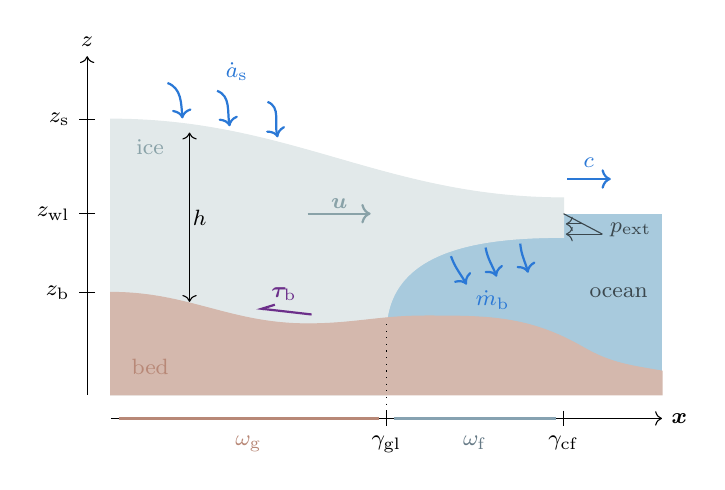
\begin{tikzpicture}[scale=1.0, every node/.style={font=\footnotesize},
    flux/.style={->, draw=blue_custom, thick},
    vec/.style={->, draw=black, thick}]

    % --- bodies -------------------------------------------------------------------------------------------
    % ocean (and cavity), up to the water level z_wl = 2.3
    \draw[draw=none, fill=color_sea] (0, 0) -- (0, 2.3) -- (7.0, 2.3) -- (7.0, 0) -- cycle;
    % ice: upper surface z_s, calving cliff at x = 5.75, lower surface z_l back to the grounding line
    \draw[draw=color_ice!150, fill=color_ice!150] (0, 0) -- (0, 3.5) to[out=0, in=180] (5.75, 2.5) -- (5.75, 2) to[out=-180, in=85] (3.5, 0.9) -- (3.5, 0) -- cycle;
    % bedrock z_b
    \draw[draw=color_bed!60, fill=color_bed!60] (0, 0) -- (0, 1.3) to[out=0, in=180] (2.5, 0.9) to[out=0, in=180] (4, 1.0) to[out=0, in=150] (6, 0.6) to[out=-30, in=170] (7.0, 0.3) -- (7.0, 0) -- cycle;

    % --- labels of the bodies --------------------------------------------------------------------------------
    \node[color_bed] at (0.5, 0.35) {bed};
    \node[color_ice!620] at (0.5, 3.15) {ice};
    \node[color_sea!35!black] at (6.45, 1.3) {ocean};

    % --- surfaces ------------------------------------------------------------------------------------------
    \draw (-0.2, 1.3) -- (-0.4, 1.3) node[left] {$z\basal$};
    \draw (-0.2, 2.3) -- (-0.4, 2.3) node[left] {$z\wl$};
    \draw (-0.2, 3.5) -- (-0.4, 3.5) node[left] {$z\surf$};
    % thickness
    \draw[<->] (1.0, 1.18) -- (1.0, 3.33);
    \node[right, inner sep=1pt] at (1.0, 2.25) {$h$};

    % --- grounding line and calving front --------------------------------------------------------------------
    \draw[dotted, thin] (3.5, 0.9) -- (3.5, -0.2);

    % --- flow, stresses and mass fluxes ----------------------------------------------------------------------
    \draw[->, thick, draw=color_ice!620] (2.5, 2.3) -- (3.3, 2.3);
    \node[color_ice!620, above, inner sep=1pt] at (2.9, 2.32) {$\bm{u}$};
    % basal drag on the grounded part
    \draw[color_flat, thick, -{Straight Barb[right, length=1.6mm, width=1.4mm]}] (2.55, 1.02) -- (1.85, 1.10);
    \node[color_flat, above, inner sep=1pt] at (2.2, 1.15) {$\bm{\tau}\basal$};
    % surface mass balance
    \draw[flux] (0.72, 3.96) to[out=-20, in=95] (0.91, 3.51);
    \draw[flux] (1.35, 3.86) to[out=-20, in=100] (1.51, 3.41);
    \draw[flux] (1.99, 3.72) to[out=-20, in=105] (2.12, 3.27);
    \node[blue_custom, above, inner sep=1pt] at (1.6, 3.95) {$\dot{a}\surf$};
    % sub-shelf melt (and ocean circulation in the cavity)
    \draw[->, draw=blue_custom, thick] (4.32, 1.76) to[out=-70, in=120] (4.52, 1.40);
    \draw[->, draw=blue_custom, thick] (4.76, 1.87) to[out=-80, in=110] (4.90, 1.50);
    \draw[->, draw=blue_custom, thick] (5.20, 1.92) to[out=-85, in=105] (5.30, 1.55);
    \node[blue_custom, inner sep=1pt] at (4.85, 1.2) {$\dot{m}\basal$};
    % calving and frontal melt
    \draw[flux] (5.8, 2.74) -- (6.35, 2.74);
    \node[blue_custom, above, inner sep=1pt] at (6.07, 2.84) {$c$};
    % hydrostatic pressure on the submerged face
    \foreach \z in {2.17, 2.04} {\pgfmathsetmacro{\len}{1.9*(2.3-\z)}
        \draw[->, draw=color_sea!35!black] (5.75+\len, \z) -- (5.78, \z);}
    \draw[color_sea!35!black] (5.75, 2.3) -- (5.75+1.9*0.26, 2.04);
    \node[color_sea!35!black, right, inner sep=1pt] at (6.3, 2.1) {$p\ext$};

    % --- axes and footprints ---------------------------------------------------------------------------------
    \draw[->] (0, -0.3) -- ++(7.0, 0) node[right] {$\bm{x}$};
    \draw[->] (-0.3, 0) -- ++(0, 4.3) node[above] {$z$};
    \draw (3.5, -0.2) -- (3.5, -0.4) node[below] {$\gamma\gl$};
    \draw (5.75, -0.2) -- (5.75, -0.4) node[below] {$\gamma\cf$};
    \draw[color_bed, very thick] (0.1, -0.3) -- (3.4, -0.3);
    \node[color_bed, below] at (1.75, -0.4) {$\omega\gr$};
    \draw[color_sea!80!black, very thick] (3.6, -0.3) -- (5.65, -0.3);
    \node[color_sea!60!black, below] at (4.625, -0.4) {$\omega\fl$};
\end{tikzpicture}

\end{document}
